\documentclass[a4paper,12pt]{article}
\usepackage{graphicx}
\usepackage[UTF8]{ctex}
\usepackage{fontspec}
\usepackage{booktabs}
\usepackage{float}%浮动体
\usepackage{amsmath,amssymb}
\usepackage{fancyhdr}
%\usepackage{xcolor}
\usepackage{colortbl}
\usepackage{geometry}
\geometry{top=2cm,bottom=2cm,left=1cm,right=1cm}
\begin{document}
	\begin{figure}[H]
	\begin{center}
		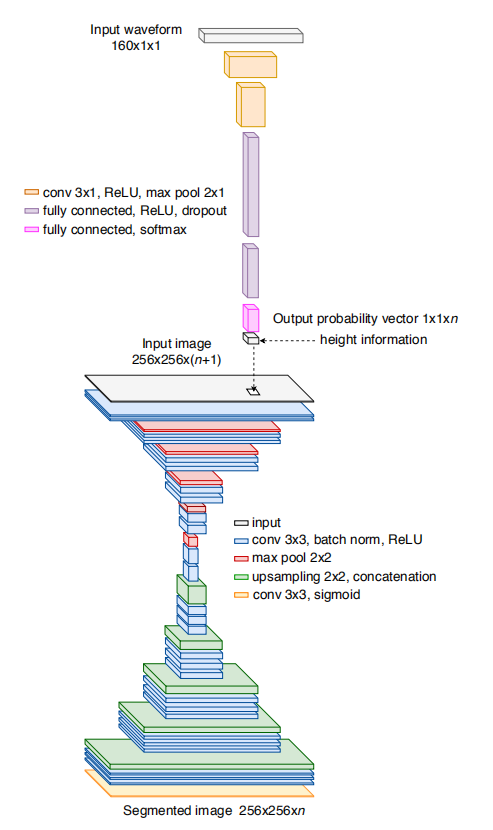
\includegraphics[width=0.6\textwidth]{img/LiDaCNN.png} 
		\caption{LiDaCNN}
	\end{center}
\end{figure}


\textbf{分析}:
\begin{itemize}
	\item 先用waveform对该点进行初始的分类。
	\item 将点云投影到一张256x256的图片中,channel包括n个分类点的概率,还有1个高度信息(256x256xn+1)
\end{itemize}

\paragraph{语义分割} 如图1,反卷积和跳跃连接将像素还原,然后对每个像素点进行分类。\\
\textbf{不足:}可能两个点投影在同一个像素上,但是这两个点属于不同的类别
\end{document}